\chapter{Transformer模型的搭建与训练}

\section{ 神经网络的结构}

\begin{figure}[h]
	\centering
	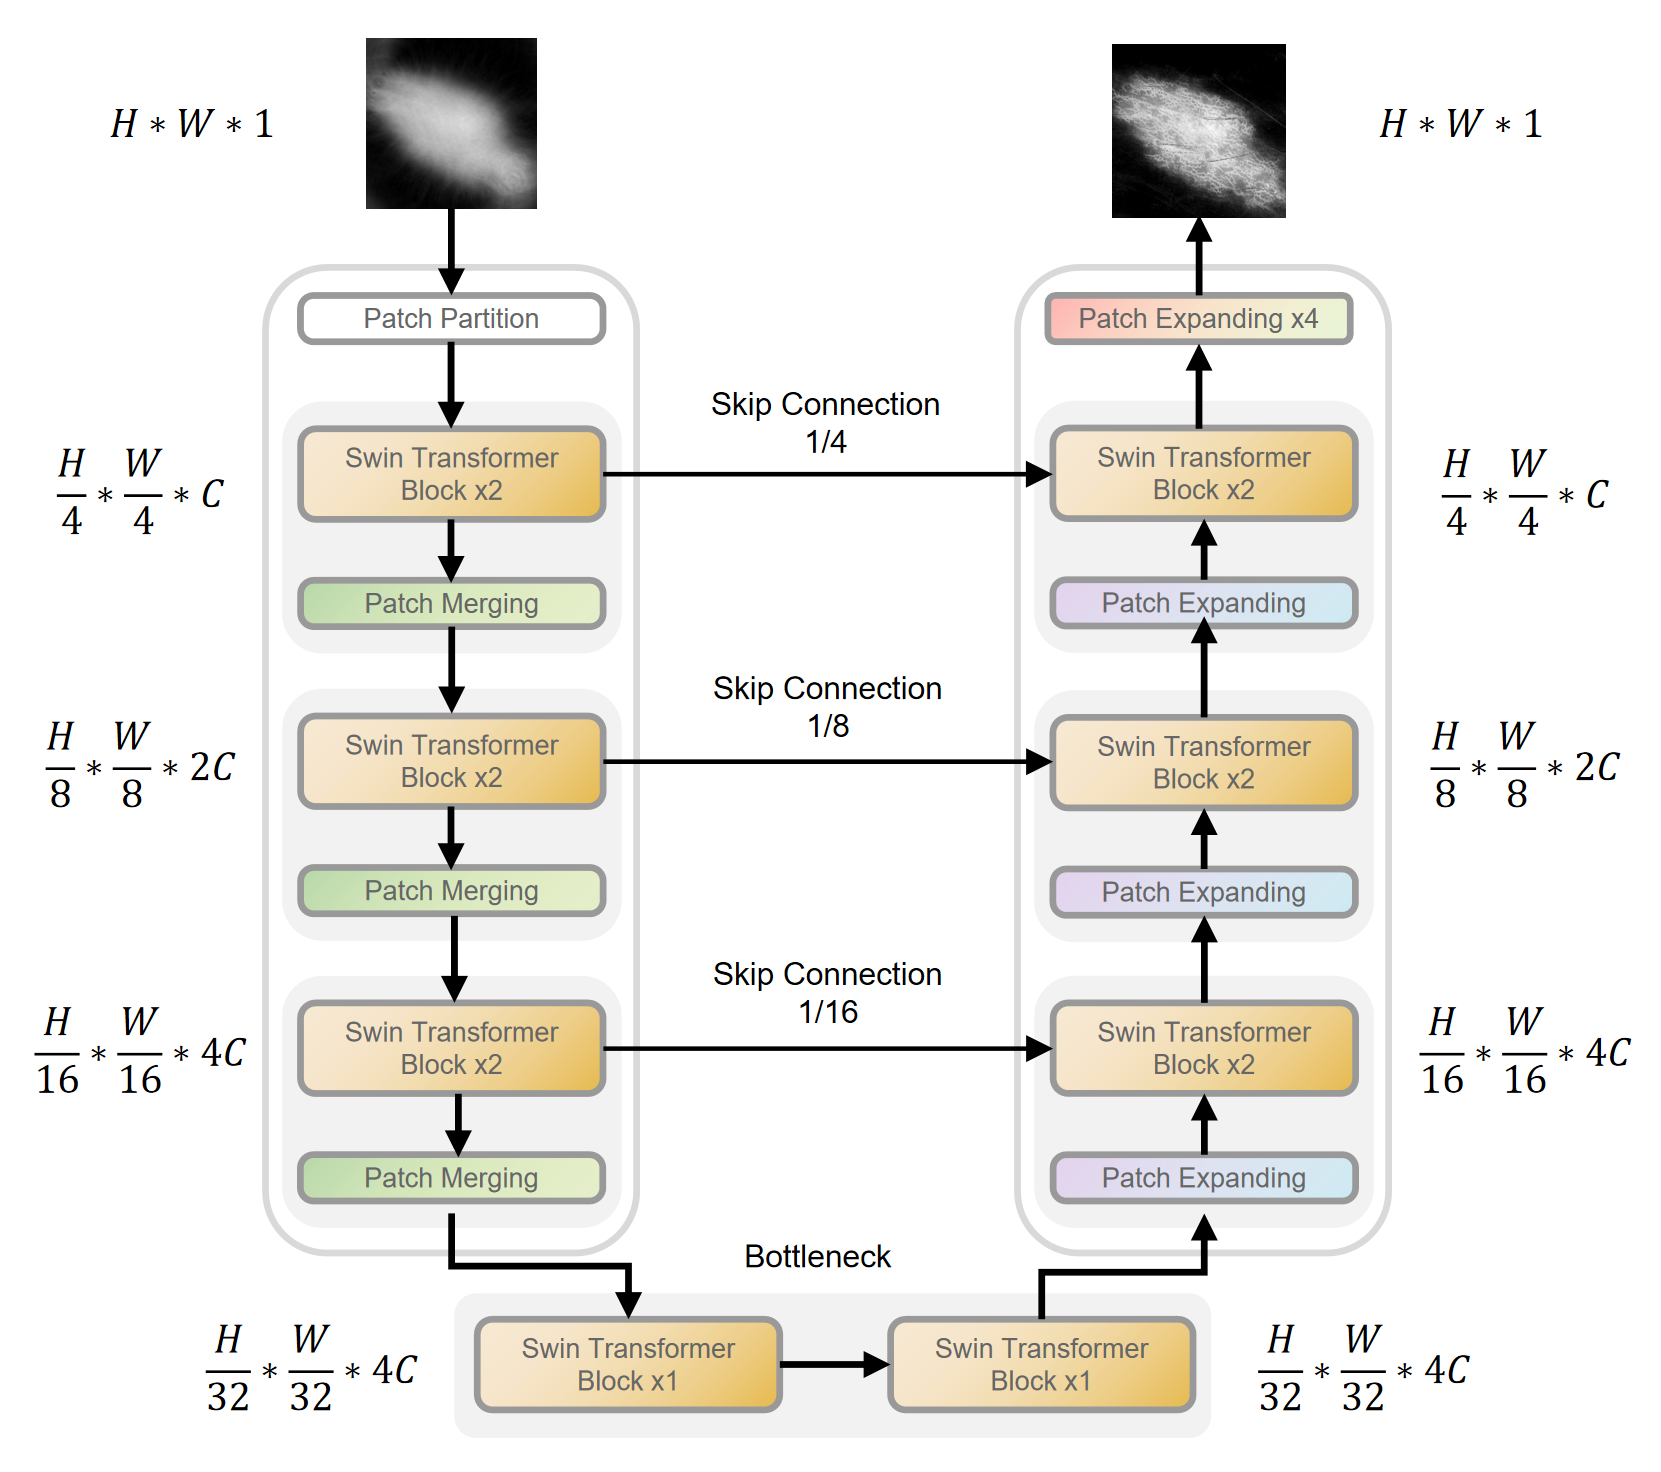
\includegraphics[width=0.9\columnwidth]{image/chap05/img501.png}
	\caption{神经网络的结构}
	\label{img501}
\end{figure}

如图\ref{img501},整个神经网络由左半部分的Encoder和右半部分的Decoder两部分组成。其中光声成像重建的灰度图像经过Encoder,分辨率逐层递减,通道数逐层增加;而后经过Decoder,分辨率逐层增加,通道数逐层递减,最后恢复到输入图像的通道数与分辨率;其中,Encoder和Decoder相同分辨率的tensor使用concat操作进行Skip Connection。

下面将详细阐述神经网络模型各层的实现方式与实现目的。

\section{Encoder和Decoder结构与 Long Skip Connection}
由于在实验初期,浅层神经网络对光声重建图像的优化效果并不理想,于是选择加深网络层数以达到较好的实现效果。但是深层神经网络存在两大问题:

\begin{enumerate}
	\item 加深模型的层数导致的训练模型时训练速度较慢、应用模型时推理速度较慢等问题,从而使得训练过程与部署过程面临较大困难。
	\item 随着隐藏层数量的增多,深层神经网络模型无法很好的结合浅层与深层的信息。
\end{enumerate}

为此,本项目拟采用Encoder和Decoder相结合的U型神经网络结构与深层和浅层神经网络的Skip Connection来解决以上两个问题。

\subsection{Encoder和Decoder结构}

观察到tensor的分辨率是影响神经网络模型推理速度的主要原因之一,因此本项目采用在Transformer Block之间使用降采样层的方法来降低中间过程tensor的分辨率。然后再通过上采样恢复成原图像的分辨率,最终输出优化图片。这种结构称为Encoder-Decoder架构。

这种Encoder-Decoder架构使得中间隐藏层处理的tensor的分辨率显著降低,从而达到加快模型推理速度的目的。

\subsection{Long Skip Connection}
本模型拟采用将Encoder和Decoder相同分辨率的tensor进行Skip Connection,从而达到保留浅层信息与结合浅层和深层信息的目的,提高对重建图像的优化效果。

\section{Patch Embeding、Patch Merging层、Patch Expanding层和Patch Expandx4层}

\begin{figure}[h]
	\centering
	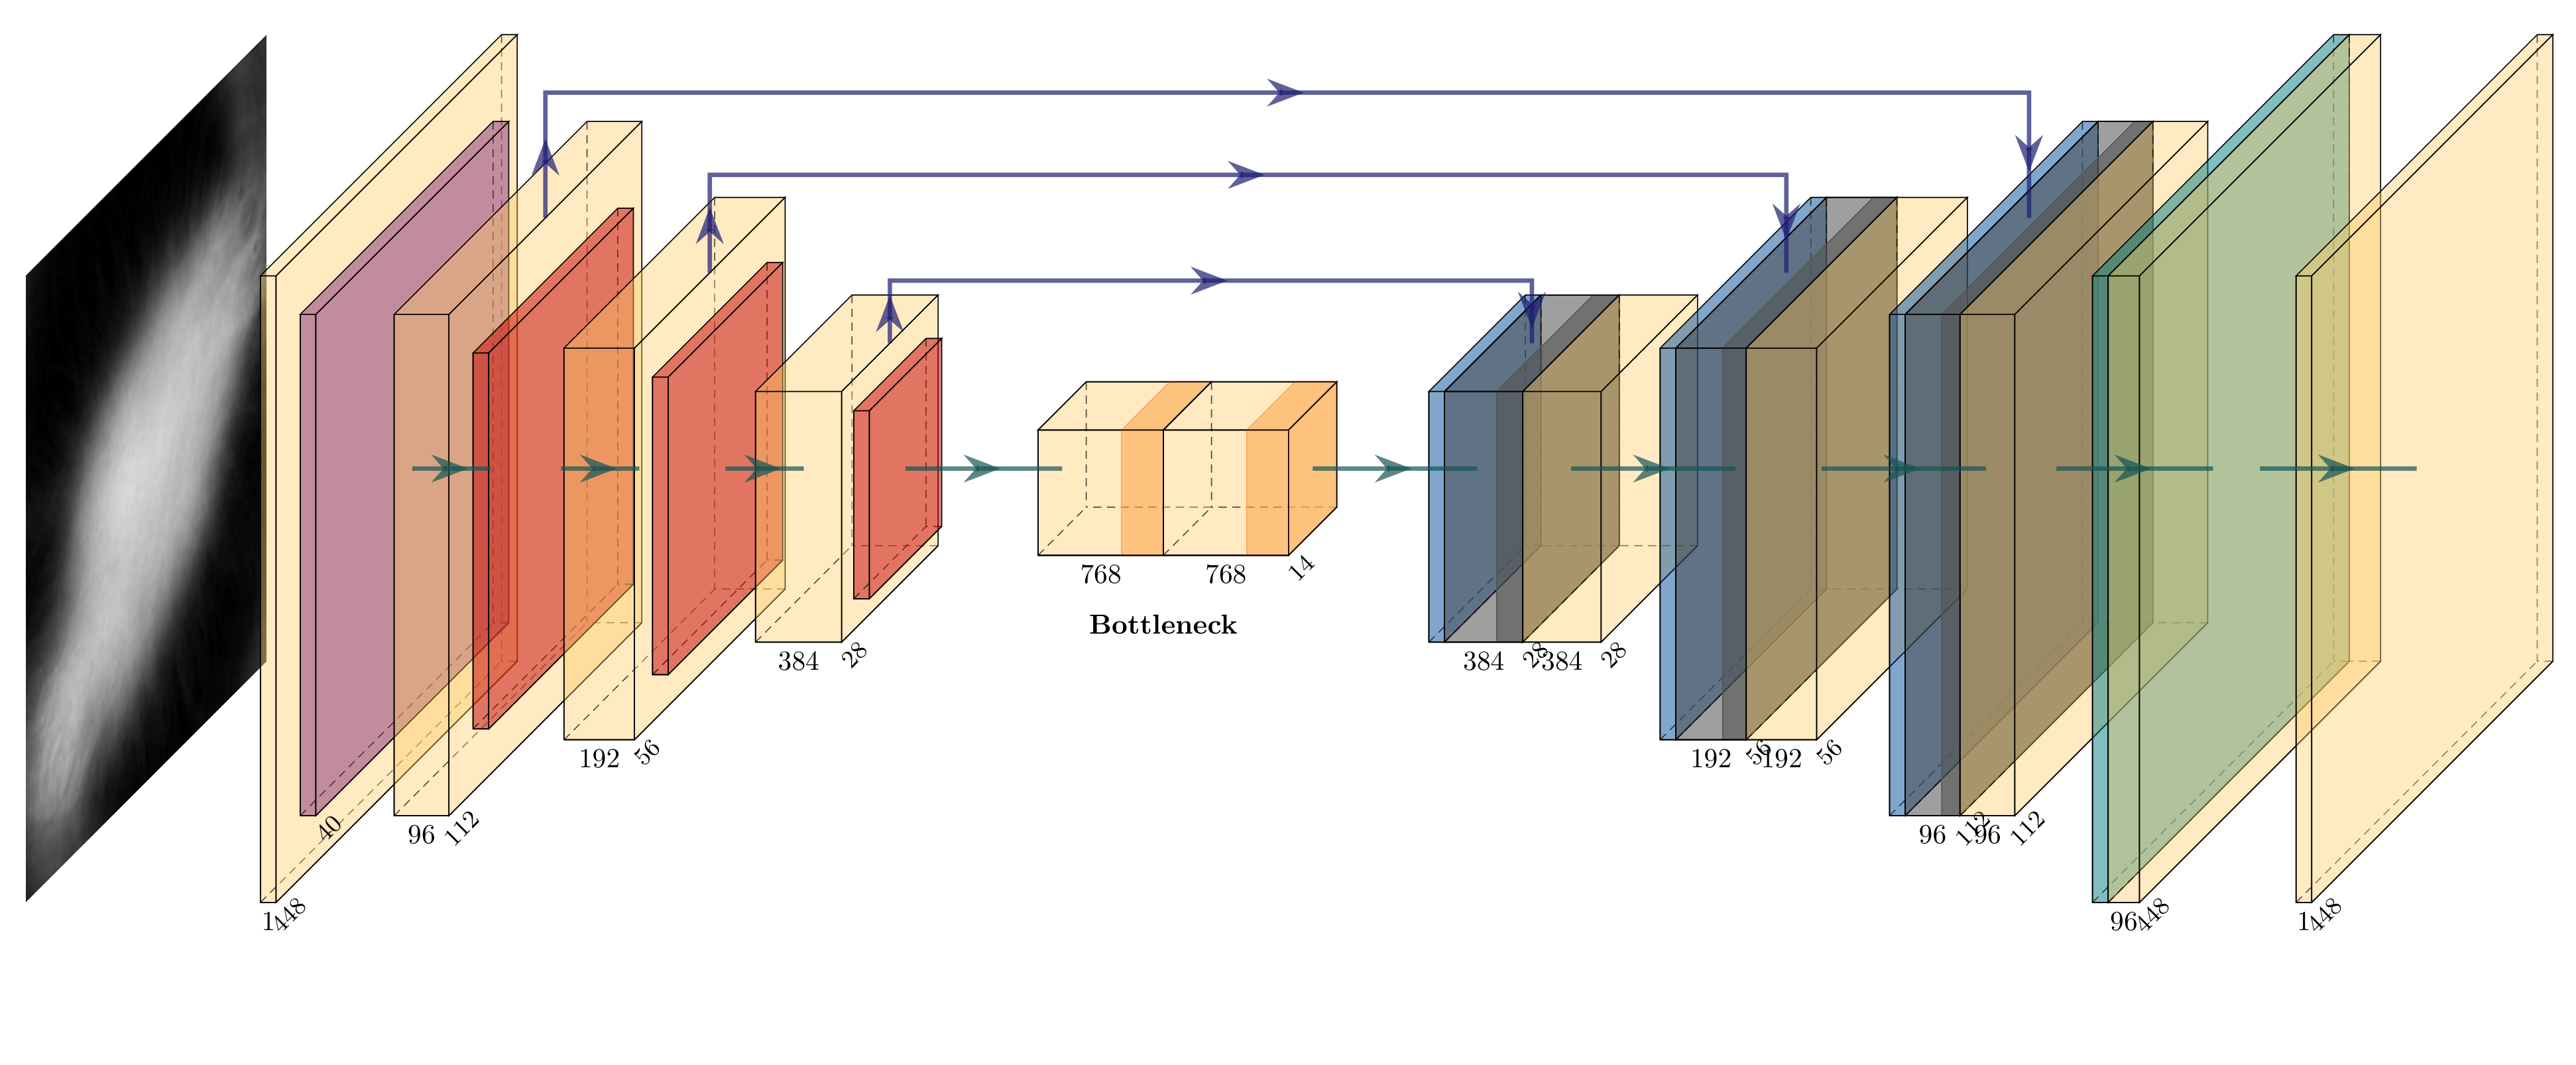
\includegraphics[width=0.9\columnwidth]{image/chap05/img502.png}
	\caption{tensor在神经网络内的形状变化}
	\label{img502}
\end{figure}

图\ref{img502}黄色层为输入、输出图片或Transformer block,紫色层为patch embeding层,红色层为Patch Merging层,蓝色层为Patch Expanding层,绿色为Patch Expandx4层。

从Transformer的推导公式中,我们知道,Transformer层不改变输入tensor的形状。于是,tensor在神经网络中的shape改变来源于Patch Embeding层、Patch Merging层、Patch Expanding层和Patch Expandx4层。图\ref{img502}展示了一张图片在神经网络中的形状变化。


\begin{enumerate}
	\item 	光声成像重建图片是灰度图片,形状为($H_0$, $W_0$, 1) = (448, 448, 1);
	\item 在经过patch embeding层(图\ref{img502}紫色层)后,H(Hight)、W(Width)变为原来的四分之一,C(Channel)变为96,即形状变为(H, W, C) = (112, 112, 96);
	\item 将patch embeding的输出作为Transformer block的输入,然后再经过Patch Merging层(图\ref{img502}红色层),H(Hight)、W(Width)变为原来的二分之一,C(Channel)变为原来的二倍。即:
	
	\begin{table}[h]
		\caption{Patch Merging的形状变化}
		\begin{tabular}{c|ccc}
			\midrule
			\multicolumn{1}{l|}{} & \textbf{Patch Merging 1}                                             & \textbf{Patch Merging 2}                                             & \cellcolor[HTML]{FFFFFF}\textbf{Patch Merging 3}                     \\ \midrule
			\textbf{Input Shape}  & \begin{tabular}[c]{@{}c@{}}(H,W,C)\\ =(112,112,96)\end{tabular}      & \begin{tabular}[c]{@{}c@{}}(H/2,W/2,2*C)\\ =(56,56,192)\end{tabular} & \begin{tabular}[c]{@{}c@{}}(H/4,W/4,4*C)\\ =(28,28,384)\end{tabular} \\ \hline
			\textbf{Output Shape} & \begin{tabular}[c]{@{}c@{}}(H/2,W/2,2*C)\\ =(56,56,192)\end{tabular} & \begin{tabular}[c]{@{}c@{}}(H/4,W/4,4*C)\\ =(28,28,384)\end{tabular} & \begin{tabular}[c]{@{}c@{}}(H/8,W/8,8*C)\\ =(14,14,768)\end{tabular} \\ \midrule
		\end{tabular}
	\end{table}

	\item 由于Bottleneck是两个Transformer block串联而成,所以不会改变tensor的形状。
	
	\item Bottleneck的输出经过Patch Expanding层(图\ref{img502}蓝色层),H(Hight)、W(Width)变为原来的二倍,C(Channel)变为原来的二分之一。即:
	
	\begin{table}[h]
		\caption{Patch Expanding的形状变化}
		\begin{tabular}{c|ccc}
			\midrule
			\multicolumn{1}{l|}{} & \textbf{Patch Expanding 1}                                           & \textbf{Patch Expanding 2}                                           & \cellcolor[HTML]{FFFFFF}\textbf{Patch Expanding 3}                   \\ \midrule
			\textbf{Input Shape}  & \begin{tabular}[c]{@{}c@{}}(H/8,W/8,8*C)\\ =(14,14,768)\end{tabular} & \begin{tabular}[c]{@{}c@{}}(H/4,W/4,4*C)\\ =(28,28,384)\end{tabular} & \begin{tabular}[c]{@{}c@{}}(H/2,W/2,2*C)\\ =(56,56,192)\end{tabular} \\ \hline
			\textbf{Output Shape} & \begin{tabular}[c]{@{}c@{}}(H/4,W/4,4*C)\\ =(28,28,384)\end{tabular} & \begin{tabular}[c]{@{}c@{}}(H/2,W/2,2*C)\\ =(56,56,192)\end{tabular} & \begin{tabular}[c]{@{}c@{}}(H,W,C)\\ =(112,112,96)\end{tabular}      \\ \midrule
		\end{tabular}
	\end{table}
	
	\item 输出tensor经过Patch Expandx4层(图\ref{img502}绿色层),H(Hight)、W(Width)变为原来的四倍,C(Channel)数不变,即形状由(H, W, C) = (112, 112, 96)变为(448,448,96);
	
	\item 最后通过一层卷积层,将通道(Channel)数恢复为1,即形状由(448,448,96)变为(448,448,1)作为神经网络的输出

\end{enumerate}

下文详细阐述Patch Embeding层、Patch Merging层、Patch Expanding层和Patch Expandx4层的实现原理:

\subsection{Patch Embeding层}
Patch Embeding层由一个卷积核大小为4*4,卷积核个数为96,步长为4的卷积层组成。它能将输入的灰度图片的H(Hight)、W(Width)变为原来的四分之一,C(Channel)变为96。

\subsection{Patch Merging层}

\begin{figure}[h]
	\centering
	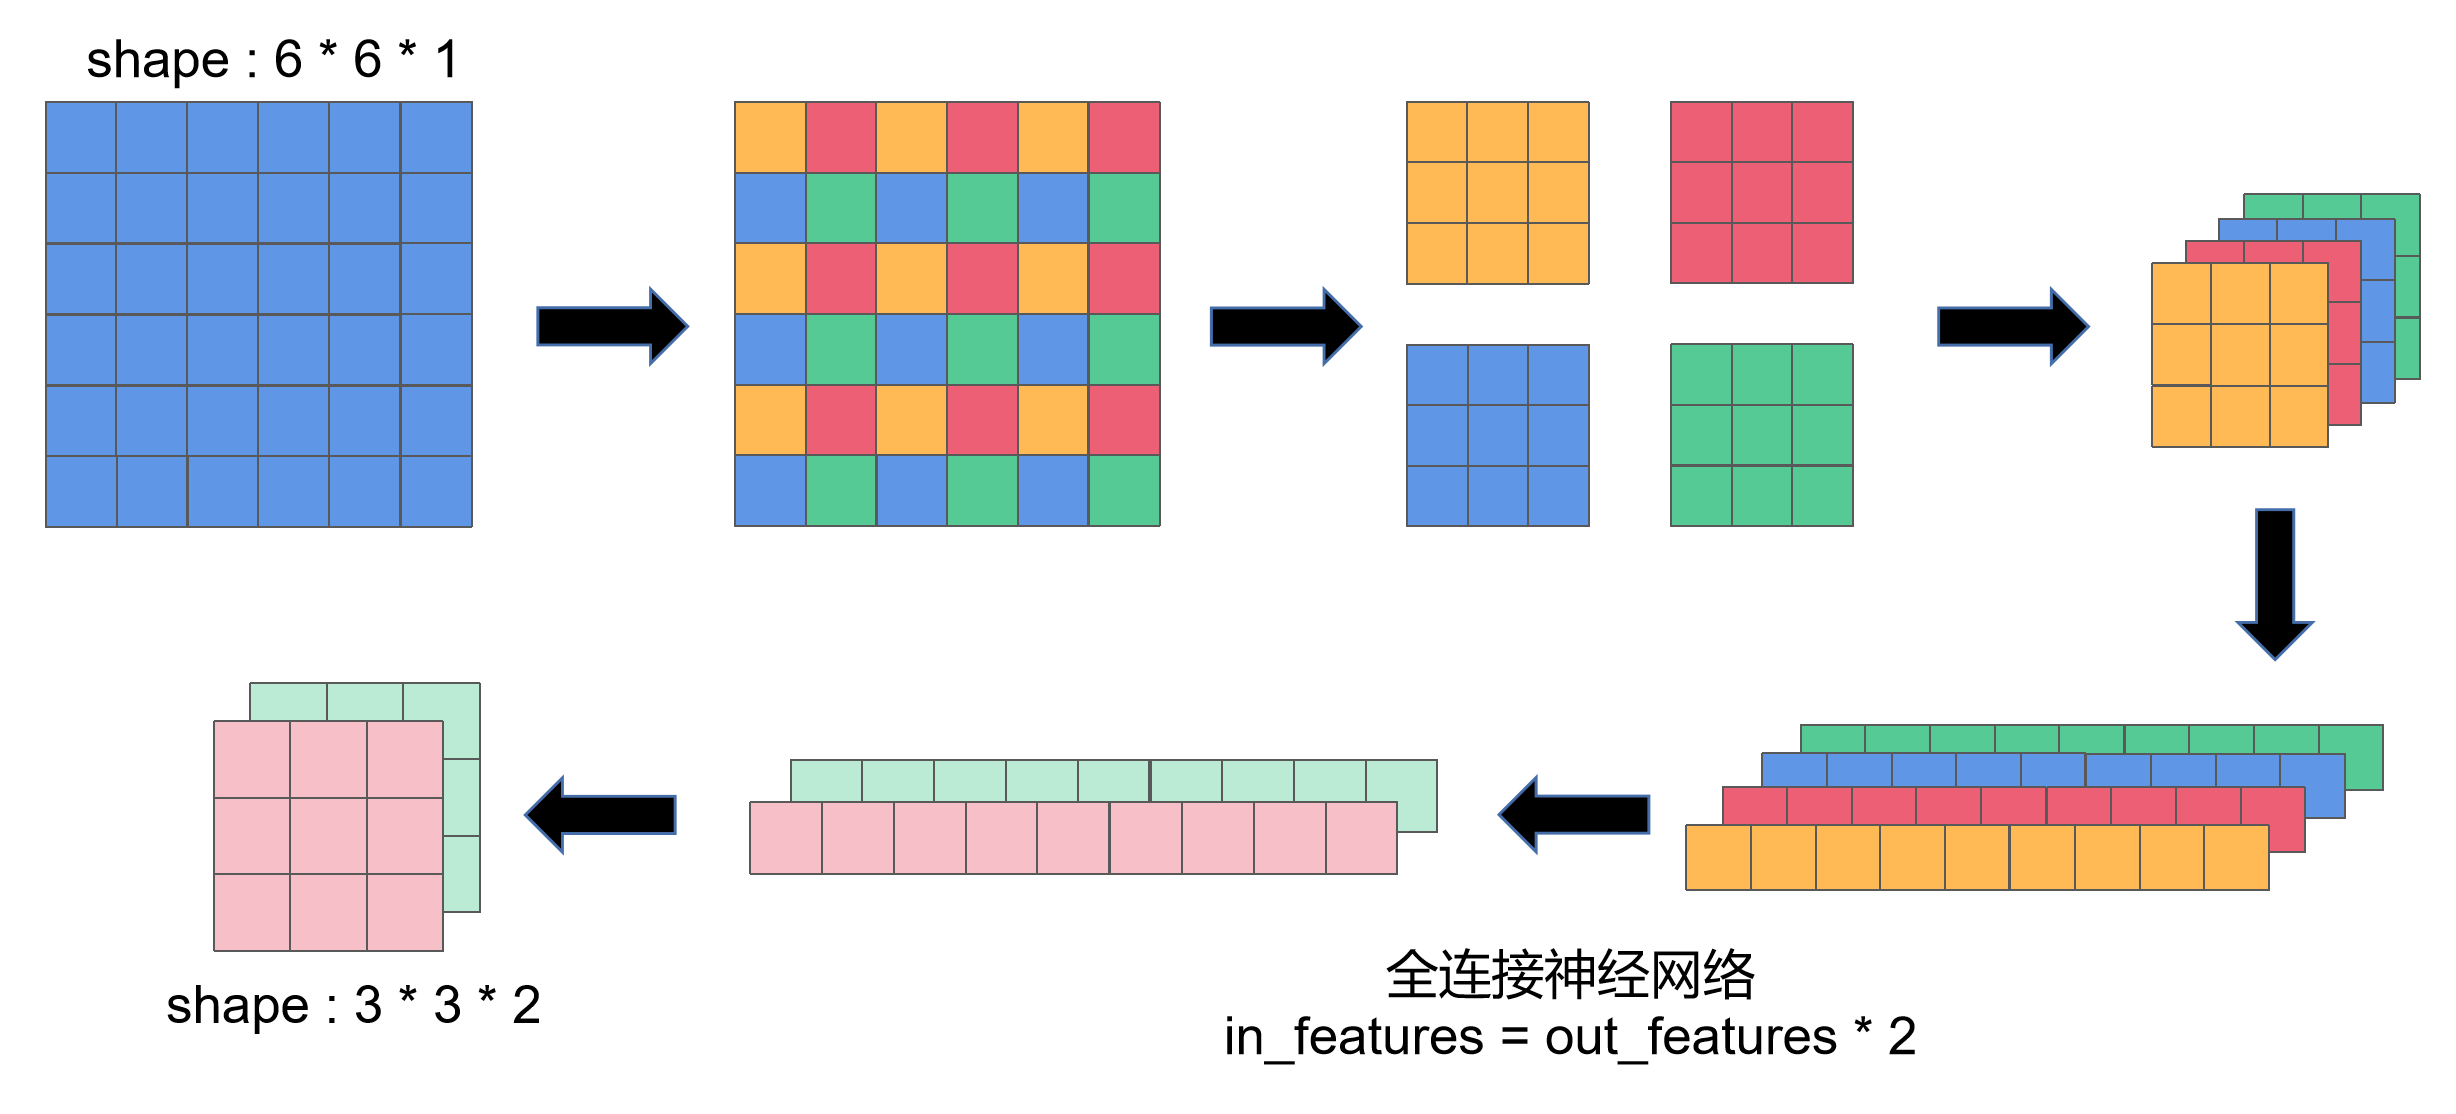
\includegraphics[width=0.9\columnwidth]{image/chap05/img503.png}
	\caption{Patch Merging的实现原理}
	\label{img503}
\end{figure}

Patch Merging层的原理如图\ref{img503}所示,它能将输入tensor的H(Hight)、W(Width)变为原来的二分之一,C(Channel)变为原来的二倍。

\subsection{Patch Expanding层}
对于形状为[B, H, W, C]的输入tensor,Patch Expanding采用的是将通道数C翻倍的线性层,将tensor的形状改变为[B, H, W, 2*C]。
然后通过使用einops库中的rearrange函数将输入tensor的分辨率H(Hight)、W(Width)扩展到原分辨率的2倍,并将通道数C(Channel)减小到输入维数的四分之一。即:

\begin{equation} \label{501}
	\begin{aligned}
		\Big [ B, H, W, 2*C \Big ] = & \Big [B, H, W, (p1, p2, c) \Big ]\\ 
		\rightarrow & \Big [  B, (H, p1), (W, p2), c \Big ] \\
		\rightarrow & \Big [ B, H*p1, W*p2, c \Big ] \\  = &\Big [ B, 2*H, 2*W, \cfrac{1}{4}C \Big ] \\ 
		w&here \  p1=2, p2=2, c=\cfrac{1}{4}C
	\end{aligned}
\end{equation}

\subsection{Patch Expandingx4层}
 与 Patch Expanding层所做的操作类似,不同的是Patch Expandingx4层采用的是将通道数C增加为16*C的线性层,将tensor的形状改变为[B, H, W, 16*C]。
 
 然后使用einops库中的rearrange函数进行如下操作:
 
 \begin{equation} \label{502}
 	\begin{aligned}
 		\Big [ B, H, W, 16*C \Big ] = & \Big [B, H, W, (p1, p2, c) \Big ]\\ 
 		\rightarrow & \Big [  B, (H, p1), (W, p2), c \Big ] \\
 		\rightarrow & \Big [ B, H*p1, W*p2, c \Big ] \\  = &\Big [ B, 4*H, 4*W, C \Big ] \\ 
 		w&here \  p1=4, p2=4, c=C
 	\end{aligned}
 \end{equation}
 
 从上面的tensor的形状变化过程可以看出,Patch Expanding层是将C拆分为C=2*2*(C/4),而Patch Expandingx4层是将C拆分为4*4*(C/16),然后使用rearrange方法。

\section{Swin Transformer Block}
Swin Transformer Block的内部结构如图\ref{img504}所示。

\begin{figure}[h]
	\centering
	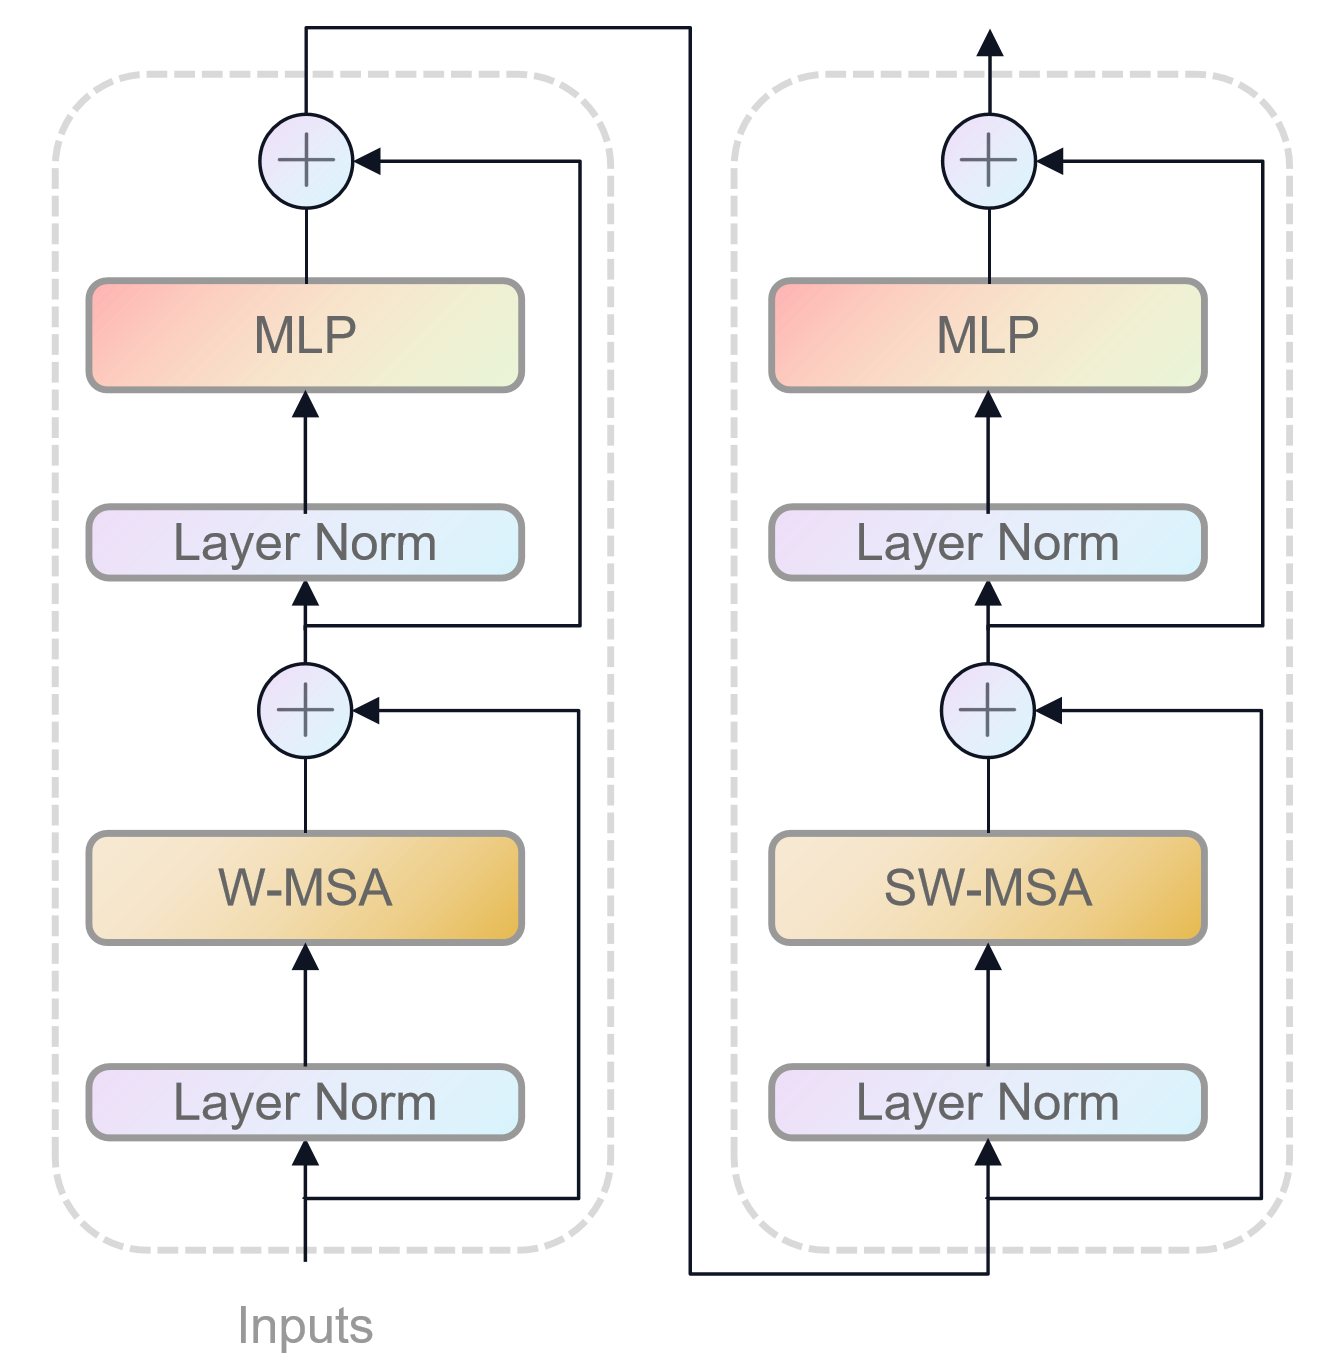
\includegraphics[width=0.65\columnwidth]{image/chap05/img504.png}
	\caption{Swin Transformer Block的结构}
	\label{img504}
\end{figure}

Swin Transformer Block中W-MASA与SW-MSA总是成对出现,先将input tensor输入到W-MSA,经过一个全连接层后,再输入到SW-MSA,最后再经过一个全连接层后输出。在上面各层之间存在Layer Normation层,且存在残差连接(Short Skip Connection)。

\subsection{Short Skip Connection}
在实验的过程中,深层神经网络往往会面临网络退化的问题。一般认为若整个网络中的部分子网络是当前最优的网络,那么更深的神经网络的其它部分只需要拟合为恒等映射 (Identity Mapping) 就可以取得与最优的网络一致的结果,因此深层网络应比浅层网络更优。但事实是由于非线性激活层的存在,深层网络难以拟合为恒等映射,从而导致网络发生退化。

相较之下,神经网络的子网络拟合为0值映射是较为容易的,因此残差单元以跳层连接的形式将单元输入直接与单元输出加在一起,神经网络拟合恒等映射等价于残差神经网络拟合 0 映射。因此能较好地解决深度网络发生退化的问题。

其次,与Long Skip Connection相对应,ResNet残差连接可以看成是一种Short Skip Connection。它同样能使得浅层信息得到更好的保留,且使得深层信息与浅层信息能得到更好的结合。

\section{模型训练结果}
在选取MSE作为损失函数后,经过200个epoch的训练,其训练集的Loss与测试集的Loss变化如图\ref{img505}所示。

\begin{figure}[h]
	\centering
	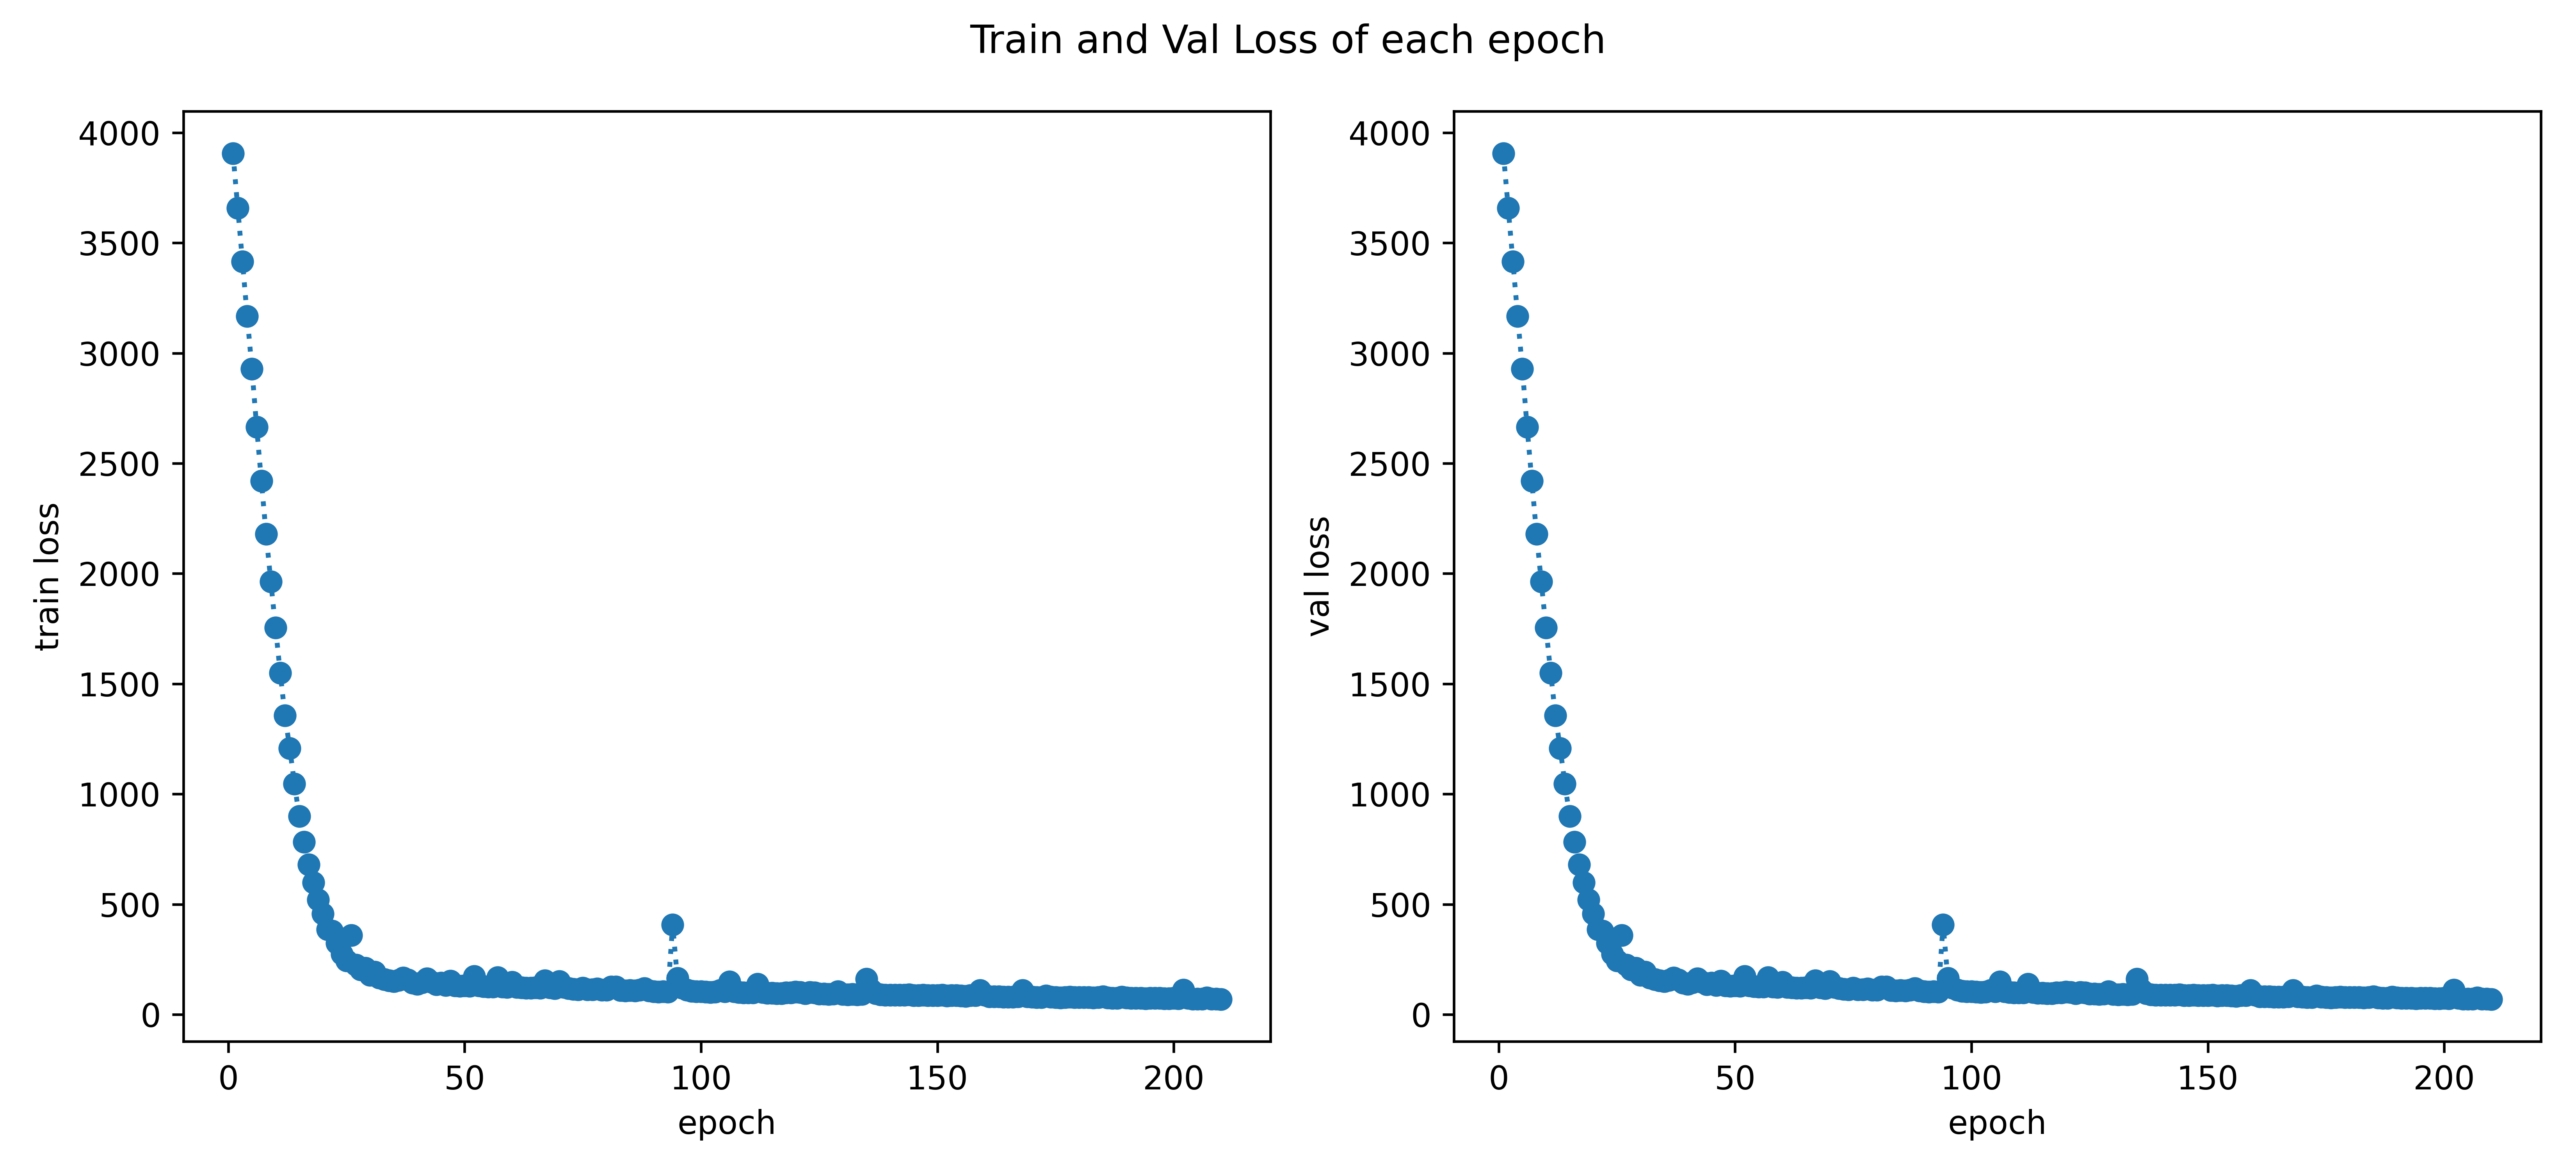
\includegraphics[width=0.9\columnwidth]{image/chap05/img505.png}
	\caption{loss随epoch的变化曲线}
	\label{img505}
\end{figure}

\hspace*{\fill} \

从Loss的变化曲线可知,模型在第1个epoch到第25个epoch,Train Loss和Val Loss都大幅度下降,最终到第200个epoch成功收敛。

将验证集(Validation Set)中抽取的两张由50个光学传感器收集数据反演所得的重建图像输入到已训练好的模型中得到预测图像。将原图像、重建图像和预测图象作图进行对比,如图\ref{img506}所示。

\begin{figure}[h]
	\centering
	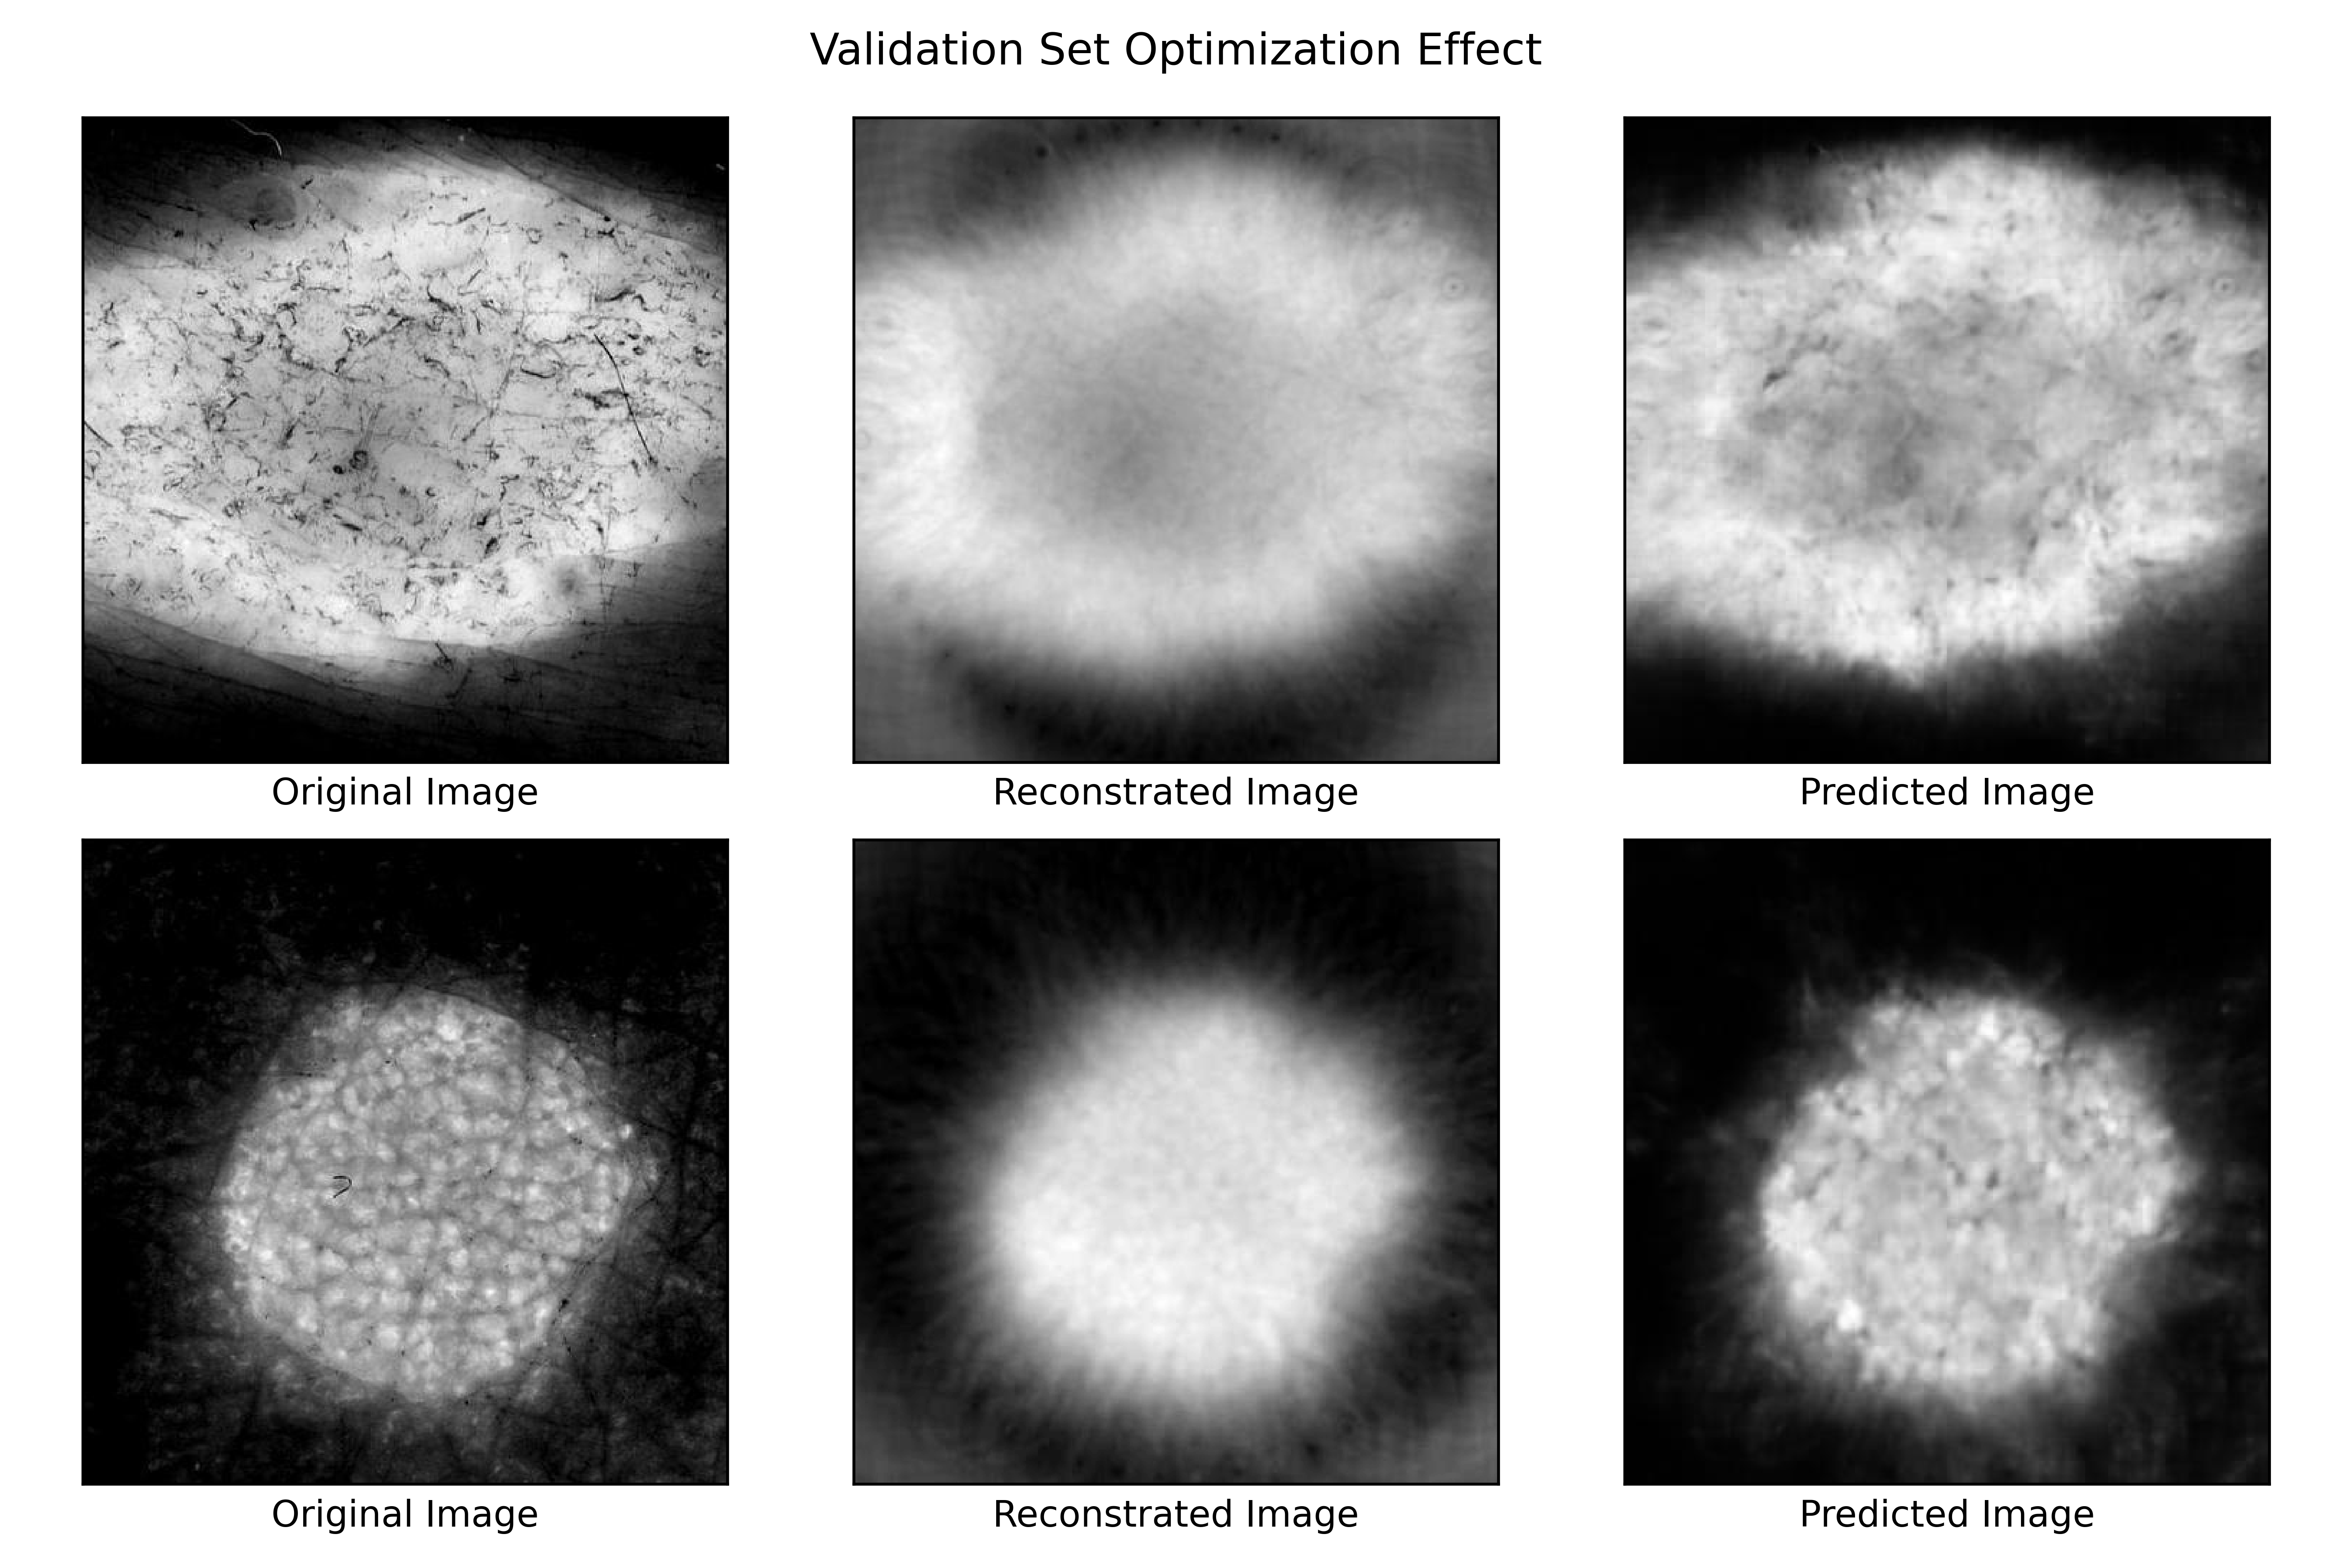
\includegraphics[width=0.9\columnwidth]{image/chap05/img506.png}
	\caption{重建图像优化效果示例}
	\label{img506}
\end{figure}

图\ref{img506}左侧图像为选定图像的原图像,中间图像为选定图像的光声重建图像,右侧图像为将重建图像输入模型所得的预测图像。从直观上可以看出,相比于光声重建图像,模型的预测图像具有更高的分辨率与对比度,且在整体和细节上更接近原图像。下面对模型的优化效果进行定量分析。
